\begin{appendices}
\chapter{Languages}\label{app:Languages}
\section{Text Corpus}\label{textcorpus}
\begin{quote}
In times past there lived a king and queen, who said to each other every day of their lives, ``Would that we had a child!" and yet they had none. But it happened once that when the queen was bathing, there came a frog out of the water, and he squatted on the ground, and said to her: ``Thy wish shall be fulfilled; before a year has gone by, thou shalt bring a daughter into the world."

And as the frog foretold, so it happened; and the queen bore a daughter so beautiful that the king could not contain himself for joy, and he ordained a great feast. Not only did he bid to it his relations, friends, and acquaintances, but also the wise women, that they might be kind and favourable to the child. There were thirteen of them in his kingdom, but as he had only provided twelve golden plates for them to eat from, one of them had to be left out.
\end{quote}

\section{English Language Table}\label{app:engtable}
Entire table of graph property values for the English word graph that was generated from the first two paragraphs of the story ``Sleeping Beauty".
\begin{figure}[H]
	\centering
	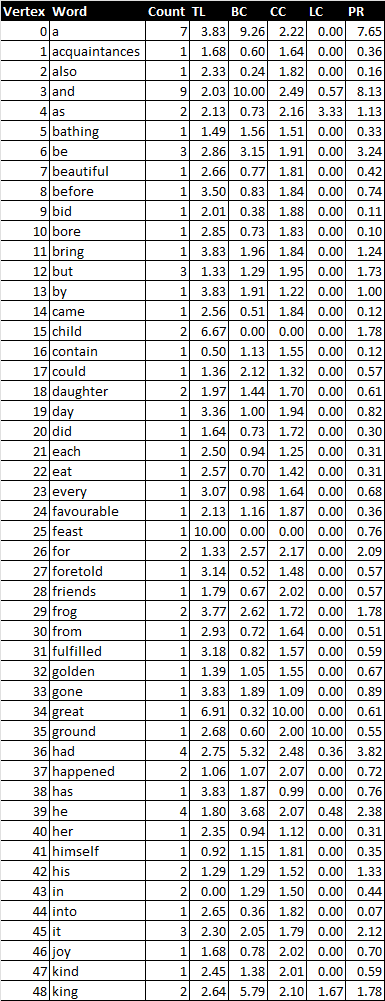
\includegraphics[scale=0.8]{engtableA.png}
\end{figure}
\begin{figure}[H]
	\centering
	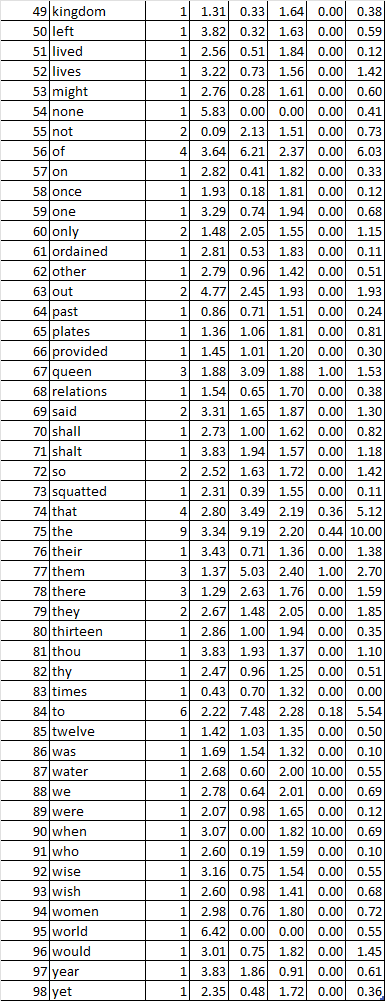
\includegraphics[scale=0.8]{engtableB.png}
\end{figure}

\section{German Language Table}\label{app:gertable}
Entire table of graph property values for the German word graph that was generated from the first two paragraphs of the story ``Sleeping Beauty".
\begin{figure}[H]
	\centering
	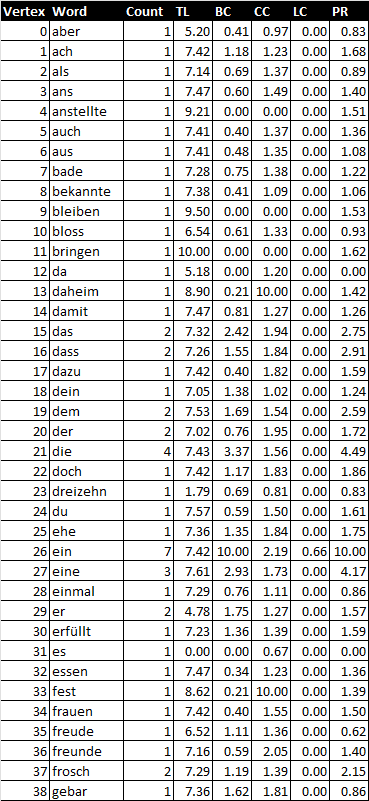
\includegraphics[scale=0.8]{gertableA.png}
\end{figure}
\begin{figure}[H]
	\centering
	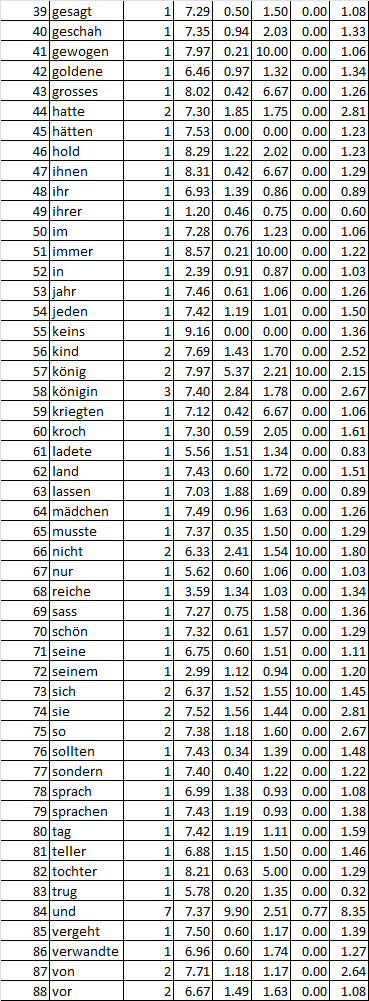
\includegraphics[scale=0.8]{gertableB.png}
\end{figure}
\begin{figure}[H]
	\centering
	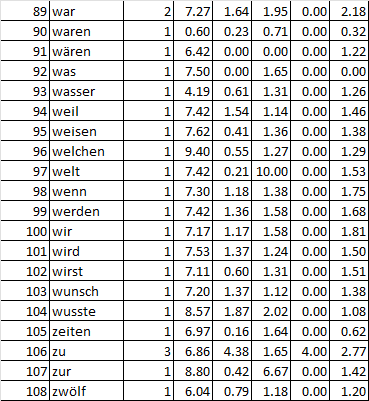
\includegraphics[scale=0.8]{gertableC.png}
\end{figure}

\newpage
\section{French Language Table}\label{app:frtable}
Entire table of graph property values for the French word graph that was generated from the first two paragraphs of the story ``Sleeping Beauty".
\begin{figure}[H]
	\centering
	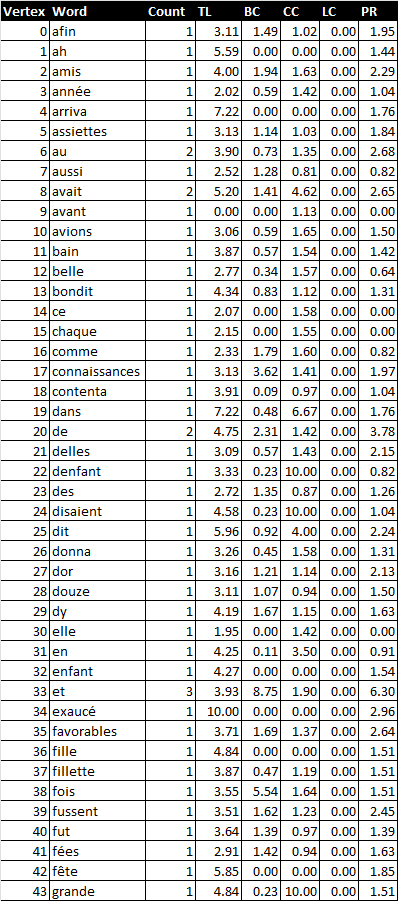
\includegraphics[scale=0.8]{frtableA.png}
\end{figure}
\begin{figure}[H]
	\centering
	\vspace{-1cm}
	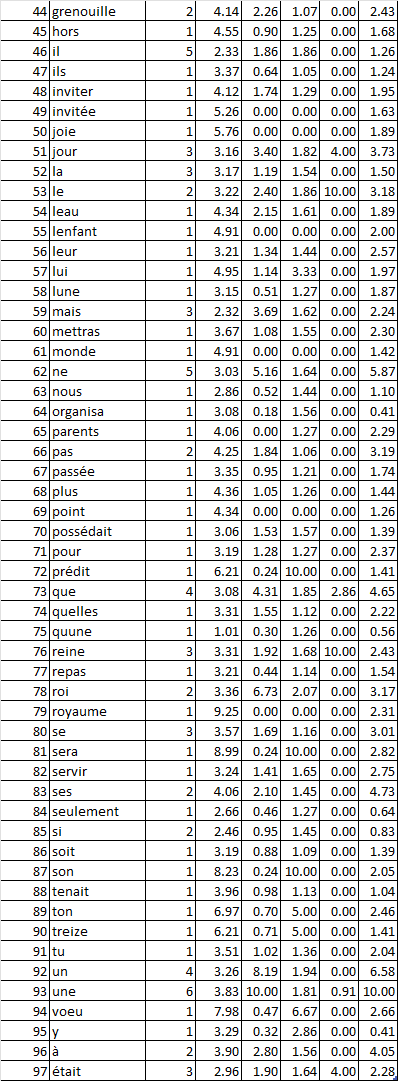
\includegraphics[scale=0.8]{frtableB.png}
\end{figure}

\newpage
\section{Japanese Language Table}\label{app:jptable}
Entire table of graph property values for the Japanese word graph that was generated from the first two paragraphs of the story ``Sleeping Beauty".
\begin{figure}[H]
	\centering
	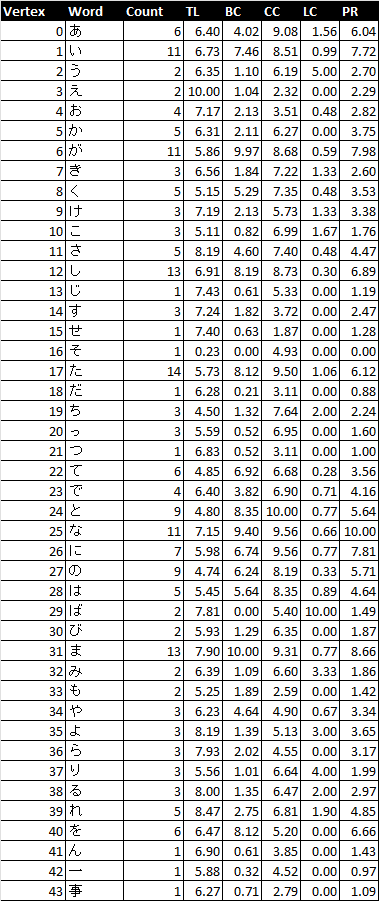
\includegraphics[scale=0.8]{jptableA.png}
\end{figure}
\begin{figure}[H]
	\centering
	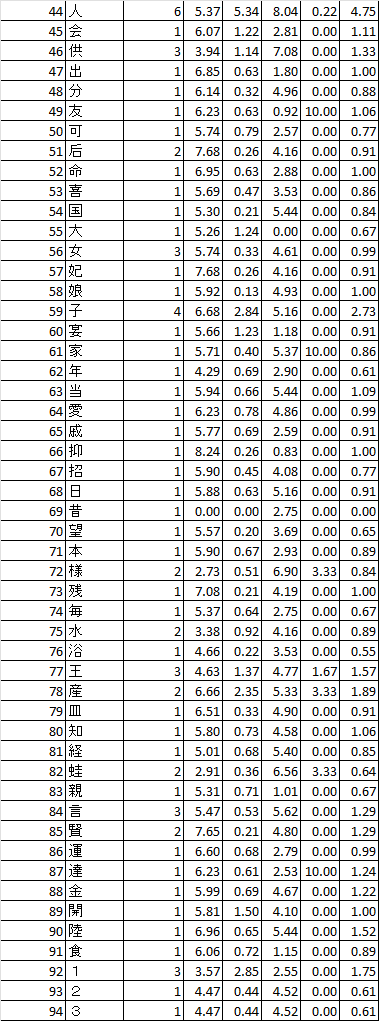
\includegraphics[scale=0.8]{jptableB.png}
\end{figure}

\newpage
\section{Chinese Language Table}\label{app:cntable}
Entire table of graph property values for the Chinese word graph that was generated from the first two paragraphs of the story ``Sleeping Beauty".
\begin{figure}[H]
	\centering
	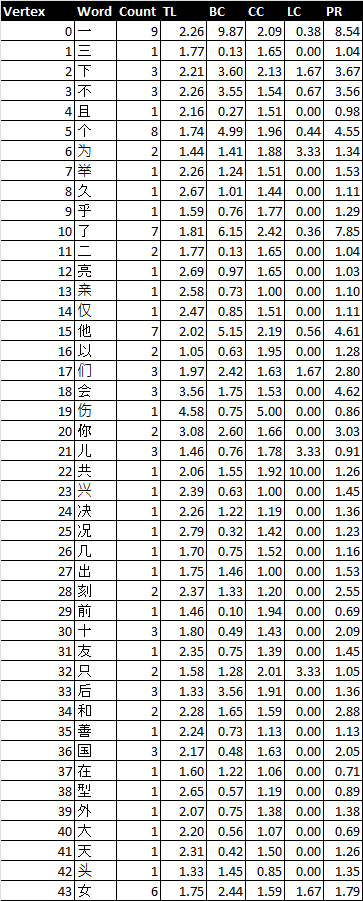
\includegraphics[scale=0.8]{cntableA.png}
\end{figure}
\begin{figure}[H]
	\centering
	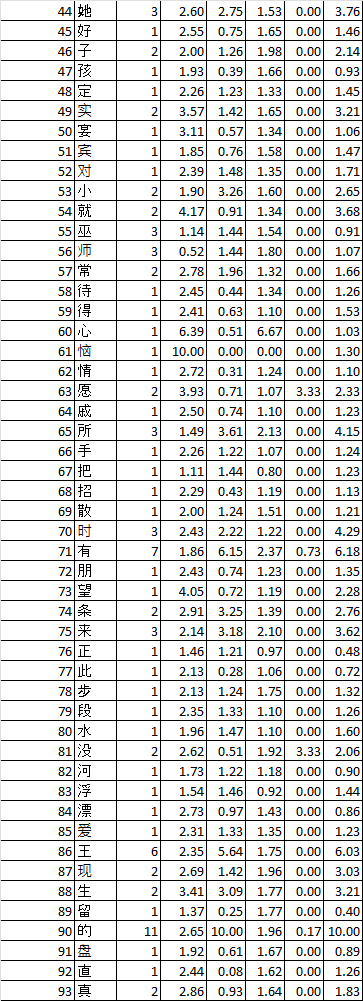
\includegraphics[scale=0.8]{cntableB.png}
\end{figure}
\begin{figure}[H]
	\centering
	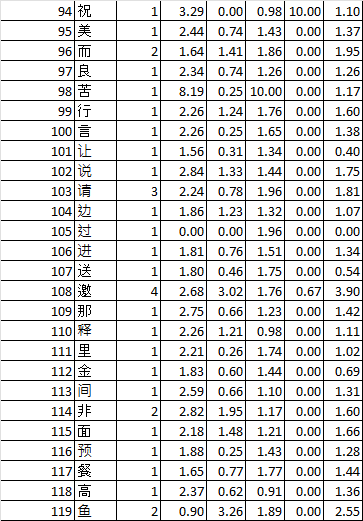
\includegraphics[scale=0.8]{cntableC.png}
\end{figure}

\end{appendices}